
\documentclass{beamer}
\usetheme{Singapore}

\setbeamertemplate{navigation symbols}{\textcolor{solarizedRebase0}{\insertframenumber}/\inserttotalframenumber}
\setbeamerfont{navigation symbols}{size=\small}

\usepackage[dark, accent=blue]{../../assets/solarized}
\usepackage{graphicx, helvet, tikz}
\usefonttheme[onlymath]{serif}

\graphicspath{{../../assets}{../images}}

\title{
    \textbf{Safer, Not Slower}\\
    ~\\
    \large Actionable insights from a large-scale survival analysis of baseball pitching mechanics
}
\author{Scott Powers}
\date{Conference on Complex Systems 2026 \\ Complexity \& Sports Satellite}

\begin{document}

  \begin{frame}[noframenumbering]
    \maketitle
    \vfill
    \hfill 
\includegraphics[width=4cm]{rice_logo_white.png}
  \end{frame}

  \begin{frame}{\bf Collaborators}
    \begin{columns}
      \begin{column}{0.33\linewidth}
        \centering
        \alert{\bf Rose Graves}\\
        Rice\\
        \vspace{1cm}
        \alert{\bf Daniel Barrueco}\\
        MLB
      \end{column}
      \begin{column}{0.33\linewidth}
        \centering
        \alert{\bf Marina Vannucci}\\
        Rice\\
        \vspace{1cm}
        \alert{\bf John D'Angelo}\\
        MLB
      \end{column}
      \begin{column}{0.33\linewidth}
        \centering
        \alert{\bf Jimmy Buffi}\\
        Reboot Motion\\
        \vspace{1cm}
        \alert{\bf Amanda Glazer}\\
        UT Austin
      \end{column}
    \end{columns}
    \vspace{1cm}
    \hfill \dots and many others!
  \end{frame}

  \begin{frame}{\bf The Problem}
    \begin{center}
      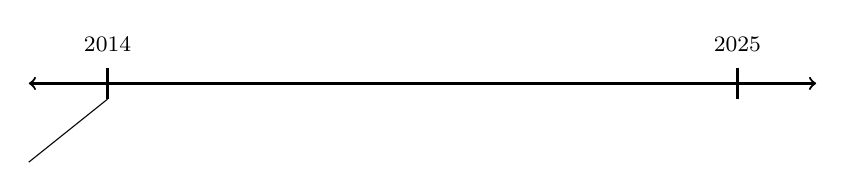
\begin{tikzpicture}
        \draw[thick, <->] (0, 0) -- (10, 0);
        \draw[thick] (1, 0.2) -- (1, -0.2);
        \node at (1, 0.5) {\footnotesize 2014};
        \draw[thick] (9, 0.2) -- (9, -0.2);
        \node at (9, 0.5) {\footnotesize 2025};
        \draw (1, -0.2) -- (0, -1);
      \end{tikzpicture}
    \end{center}
    ``From my standpoint, [Tommy John surgery] is an \alert{\bf epidemic}.''\\
    \hfill --- Dr. James Andrews\\
    \pause
    \includegraphics[width=0.95\linewidth]{injuries_by_year_dark.pdf}
  \end{frame}

  \begin{frame}{\bf 2024 MLB Report}
    \centering
    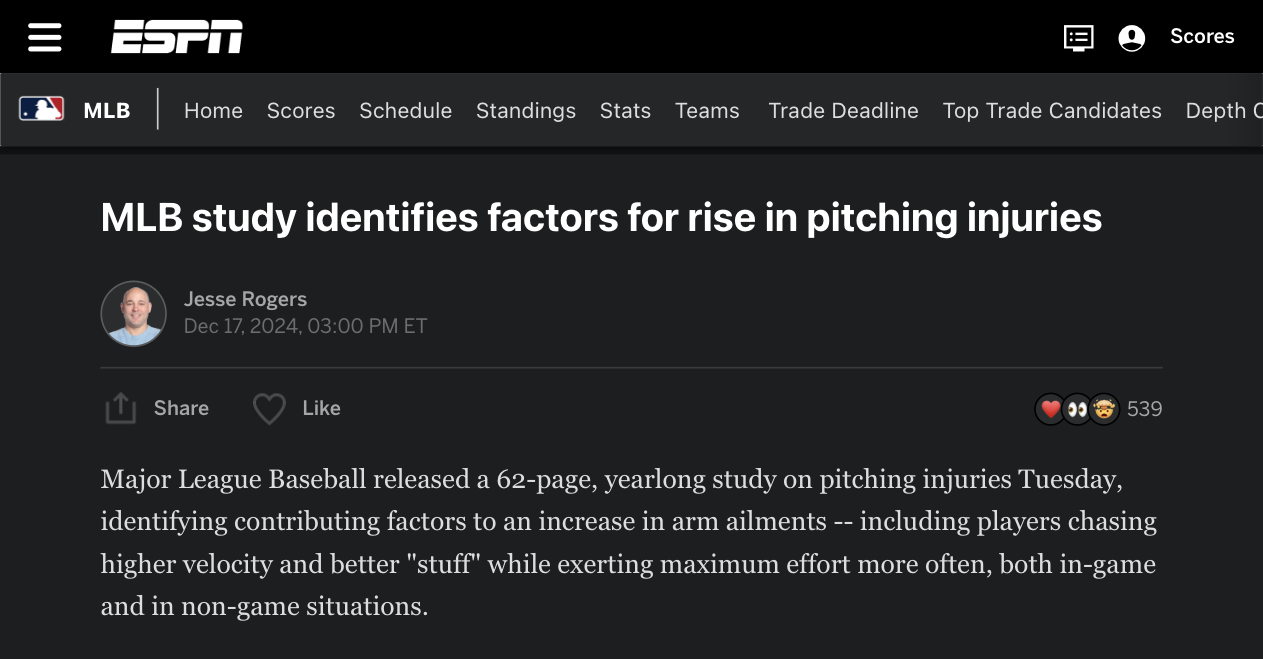
\includegraphics[width=\linewidth]{espn.png}
  \end{frame}

  \begin{frame}{\bf Data Generation}
    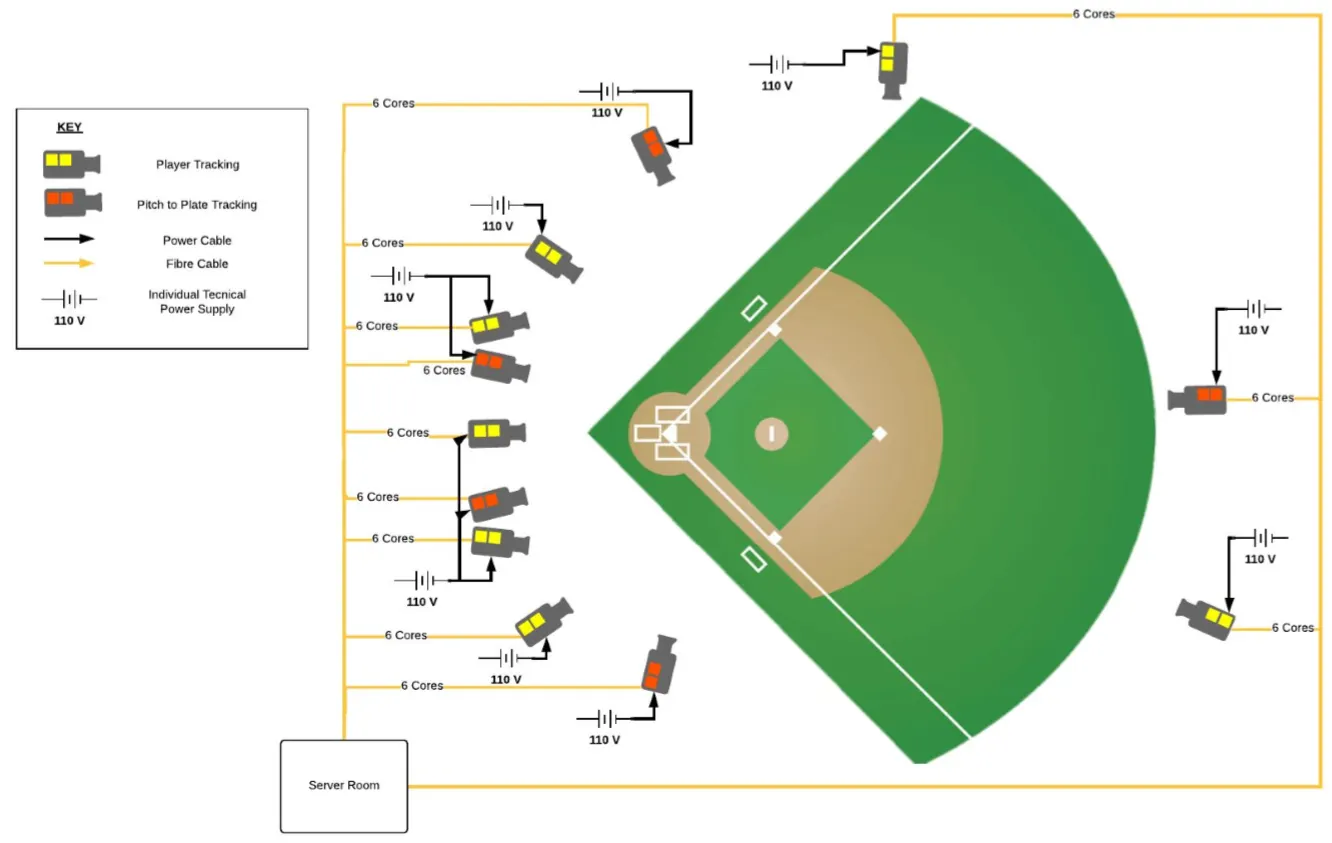
\includegraphics[width=\linewidth]{hawkeye.png}
  \end{frame}

  \begin{frame}{\bf Data}
    Pitch-by-pitch:
    \begin{itemize}
      \item ball tracking, MLB 2017+ (5,972,263 pitches)
      \item ball tracking, minors 2021+ (11,322,383 pitches)
      \item \alert{\bf skeletal pose} tracking, MLB 2023+ (1,130,824 pitches)
    \end{itemize}
    ~\\
    Injury outcomes
    \begin{itemize}
      \item 8,234 throwing-arm IL placements, MLB \& minors 2018+
      \item 1,726 (reported) UCL surgeries, MLB \& minors 2018+
    \end{itemize}
    \vfill
    \footnotesize IL = injured list \hfill UCL = ulnar collateral ligament
  \end{frame}

  \begin{frame}{\bf Methods}
    Framework:\\
    year-$Y$ features \hfill $\longmapsto$ \hfill year-($Y + 1$) pitches until IL\\
    \vfill
    Model: multivariate proportional hazards regression*
    \vfill
    Cohorts:\\
    \begin{itemize}
      \item Majors 2018--2025 (3,828 pitcher-seasons)
      \item Minors 2022--2025 (6,241 pitcher-seasons)
      \item \alert{\bf Biomechanics 2024--2025} (1,211 pitcher-seasons)
    \end{itemize}
    \vfill
    \footnotesize *clustered standard errors account for repeated pitcher observations
  \end{frame}

  \begin{frame}{\bf Pitch-Tracking Features}
    \begin{columns}
      \begin{column}{0.4\linewidth}
        Demographics
        \begin{itemize}
          \item Hand (L/R)
          \item Role (SP/RP)
          \item Past Injury (0/1)
          \item Age
        \end{itemize}
        ~\\
        Pitch Types
        \begin{itemize}
          \item SI Usage
          \item CT Usage
          \item SL+SW Usage
          \item CB+KC Usage
          \item CH+SF Usage
        \end{itemize}
      \end{column}
      \begin{column}{0.6\linewidth}
        Pitch Tracking
        \begin{itemize}
          \item Primary Velo
          \item Primary Spin Rate
          \item Lateral Release Location
          \item FB Vert Break*
          \item SL Spin Rate*
          \item CB Spin Rate*
          \item Glove-Side Break
          \item Arm-Side Break
          \item Stuff+
          \item \alert{\bf Primary Velo Effort Ratio}
        \end{itemize}
      \end{column}
    \end{columns}
    \vfill
    \footnotesize \hfill *interacted with usage
  \end{frame}

  \begin{frame}{\bf Pitch-Tracking Results}
    \hfill 95\% Conf. Int.\\
    Majors 2018--2025 cohort
    \begin{itemize}
      \item 1 mph Primary Velo $\leftrightarrow$ $+5\%$ hazard \hfill $(+2\%, +8\%)$
      \item \alert{\bf 10pp SL+SW Usage $\leftrightarrow$ $+8\%$ hazard \hfill $(+1\%, +15\%)$}
      \item 1 SD FB Vert Break $\leftrightarrow$ $+10\%$ hazard \hfill $(+3\%, +18\%)$
    \end{itemize}
    ~\\
    Minors 2022--2025 cohort
    \begin{itemize}
      \item 1 mph Primary Velo $\leftrightarrow$ $+5\%$ hazard \hfill $(+2\%, +8\%)$
      \item \alert{\bf 10pp SL+SW Usage $\leftrightarrow$ $+6\%$ hazard \hfill $(+0\%, +13\%)$}
      \item 10pp CH+SF Usage $\leftrightarrow$ $+8\%$ hazard \hfill $(+1\%, +16\%)$
      \item 1 SD Lat. Rel. Position $\leftrightarrow$ $-7\%$ hazard \hfill $(-12\%, -2\%)$
    \end{itemize}
    \vfill
    \footnotesize
    SL+SW = slider/sweeper \hfill pp = percentage point\\
    CH+SF = changeup/splitter \hfill SD = standard deviation
  \end{frame}

  \begin{frame}{\bf Compounding Risk}
    \includegraphics[width=\linewidth]{prob_injury_density_dark.pdf}\\
    Fitted injury probability* \alert{\bf varies greatly} across pitcher-seasons\\
    \vfill
    \footnotesize *Reflects 2,500-pitch starter workload or 1,000-pitch reliever workload
  \end{frame}

  \begin{frame}{\bf Biomechanics Features (Joint Angles)}
    \begin{columns}
      \begin{column}{0.34\linewidth}
        Joints:
        \begin{itemize}
          \item Rear Hip (3 df)
          \item Lead Knee (1 df)
          \item Lumbar (3 df)
          \item Shoulder (3 df)
          \item Elbow (1 df)
        \end{itemize}
      \end{column}
      \begin{column}{0.43\linewidth}
        Summary stats:
        \begin{itemize}
          \item min/max
          \item min/max timing
          \item min/max in \alert{\bf sequence}
          \item range utilization
          \item at layback
        \end{itemize}
      \end{column}
    \end{columns}
    \vfill
    \resizebox{\linewidth}{!}{
      \begin{tikzpicture}
        \draw[thick] (0, 0) -- (10, 0);
        \draw[thick] (0, 0.2) -- (0, -0.2);
        \node at (0, 0.5) {\footnotesize Foot Plant};
        \draw[thick] (10, 0.2) -- (10, -0.2);
        \node at (10, 0.5) {\footnotesize Ball Release};
        \draw[thick, solarizedBlue] (3, 0) -- (7, 0);
        \draw[thick, solarizedBlue] (3, 0.2) -- (3, -0.2);
        \draw[thick, solarizedBlue] (7, 0.2) -- (7, -0.2);
        \node at (5, 0.5) {\footnotesize \alert{\bf Sequence}};
        \node at (5, -0.7) {\footnotesize range utilization = $\frac{\text{range in sequence}}{\text{full range}}$};
        \draw[thick] (8, 0.4) -- (8, 0);
        \node at (8, 0.7) {\footnotesize Layback};
      \end{tikzpicture}
    }
    \vfill
    {\footnotesize df = degrees of freedom} \hfill \alert{\bf 67} features
  \end{frame}

  \begin{frame}{\bf Biomechanics Features (Momentum)}
    \begin{columns}
      \begin{column}{0.3\linewidth}
        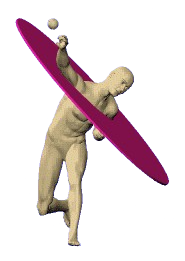
\includegraphics[width=\linewidth]{nyman.png}
        {\scriptsize from Nyman (2008)}
      \end{column}
      \begin{column}{0.27\linewidth}
        Body segments:
        \begin{itemize}
          \item Rear Leg
          \item Lead Leg
          \item Glove Arm
          \item Torso
          \item Upper Arm
          \item Forearm
          \item Hand
        \end{itemize}
      \end{column}
      \begin{column}{0.43\linewidth}
        Summary stats:
        \begin{itemize}
          \item tilt of rotation plane
          \item angular momentum projected onto plane of pitching hand (min/max, at release)
          \item angular momentum orthogonal to pitching hand plane (min/max)
        \end{itemize}
      \end{column}
    \end{columns}
    \vfill
    \hfill 67 features + \alert{\bf 72} features = 139 features
  \end{frame}

  \begin{frame}{\bf Biomechanics Suspects}
    \begin{enumerate}
      \item Max Elbow Varus Torque
      \item Arm Slot
      \item Min Shoulder Horizontal Abduction (aka scap loading)
      \item Max Glove Arm Momentum (projected onto pitching hand)
      \item Max Torso Momentum (projected onto pitching hand)
    \end{enumerate}
    \vfill
    Model: multivariate proportional hazards regression
    \begin{itemize}
      \item include demographic and significant pitch-tracking features
    \end{itemize}
  \end{frame}

  \begin{frame}{\bf Biomechanics Results}
    \begin{center}
      \begin{tabular}{l|rc}
        Feature & Effect* & 95\% Conf. Int.\\
          \hline
          Max Elbow Varus Torque & +2\% & (--8\%, +14\%)\\ 
          Arm Slot & +7\% & (--7\%, +22\%)\\ 
          Min Shoulder Horizontal Abd. & --4\% & (--14\%, +6\%)\\ 
          \alert{\bf Max Glove Arm Momentum} & \alert{\bf --21\%} & \alert{\bf (--29\%, --12\%)}\\ 
          Max Torso Momentum & +3\% & (--8\%, +16\%)\\ 
      \end{tabular}
    \end{center}
    \vfill
    \hfill \footnotesize *corresponding to 1-standard-deviation increase in feature
  \end{frame}

  \begin{frame}{\bf Data Mining}
    Model: lasso regression
    \begin{itemize}
      \item include demographic and significant pitch-tracking features
      \item include all 139 biomechanics features
      \item \alert{\bf $\ell_1$ penalty} achieves variable selection
    \end{itemize}
    \vfill
    Two outcomes: (1) pitches until IL and (2) fastball velocity
  \end{frame}

  \begin{frame}{\bf Data Mining Results}
    \begin{columns}
      \begin{column}{0.6\linewidth}
        \includegraphics[width=\linewidth]{lasso_coxph_velo_dark.pdf}
      \end{column}
      \begin{column}{0.4\linewidth}
        Glove Arm Momentum Max is the only metric associated with \alert{\bf increased} velocity and \alert{\bf decreased} injury hazard
      \end{column}
    \end{columns}
  \end{frame}

  \begin{frame}{\bf What have we learned?}
    First public study to estimate pitcher injury survival model using pitch-tracking data (\alert{\bf 20-50\%} injury probability over full season)\\
    ~\\
    Non-fastball usage (especially \alert{\bf slider/sweeper}) is positively associated with injury hazard in both MLB and minors\\
    ~\\
    \alert{\bf Glove arm momentum} is strongly predictive of reduced injury hazard (and increased velocity), warranting further research\\
    ~\\
    Notable negative findings
    \begin{itemize}
      \item Primary Velo Effort Ratio
      \item Spin Rate and Glove-Side Break
    \end{itemize}
  \end{frame}

  \begin{frame}{\bf Bayesian Changepoint Detection}
    Project led by \alert{\bf Rose Graves} (Rice Stats PhD student)\\
    ~\\
    Goal: Identify when pitchers are pitching fatigued\\
    ~\\
    Problem:
    \begin{itemize}
      \item Measurements are noisy
      \item Fatigue onset by game likely similar but not identical
    \end{itemize}
    ~\\
    Solution: Bayesian Hierarchical Changepoint model
    \begin{enumerate}
      \item Hierarchy across games within pitcher
      \item Hierarchy across pitchers within league
    \end{enumerate}
  \end{frame}

  \begin{frame}{\bf Changepoint Causal Inference}
    Project led by \alert{\bf Amanda Glazer} (University of Texas)\\
    ~\\
    Goal: Estimate causal effect of velocity increase\\
    ~\\
    Problem:
    \begin{itemize}
      \item Rolling ``enrollment'' in treatment
      \item No treatment labels in the data
    \end{itemize}
    ~\\
    Solution:
    \begin{enumerate}
      \item Identify statistically significant changepoints
      \item Perform rolling treatment-control matching
    \end{enumerate}
  \end{frame}

  \begin{frame}{\bf Shear Wave Elastography}
    Collaboration with \alert{\bf Dr. Robert Jack} (Houston Methodist)\\
    ~\\
    Problem: Not enough pitching injuries!\\
    ~\\
    Solution: Measure laxity of UCL after pitching (pilot study)\\
    ~\\
    \centering
    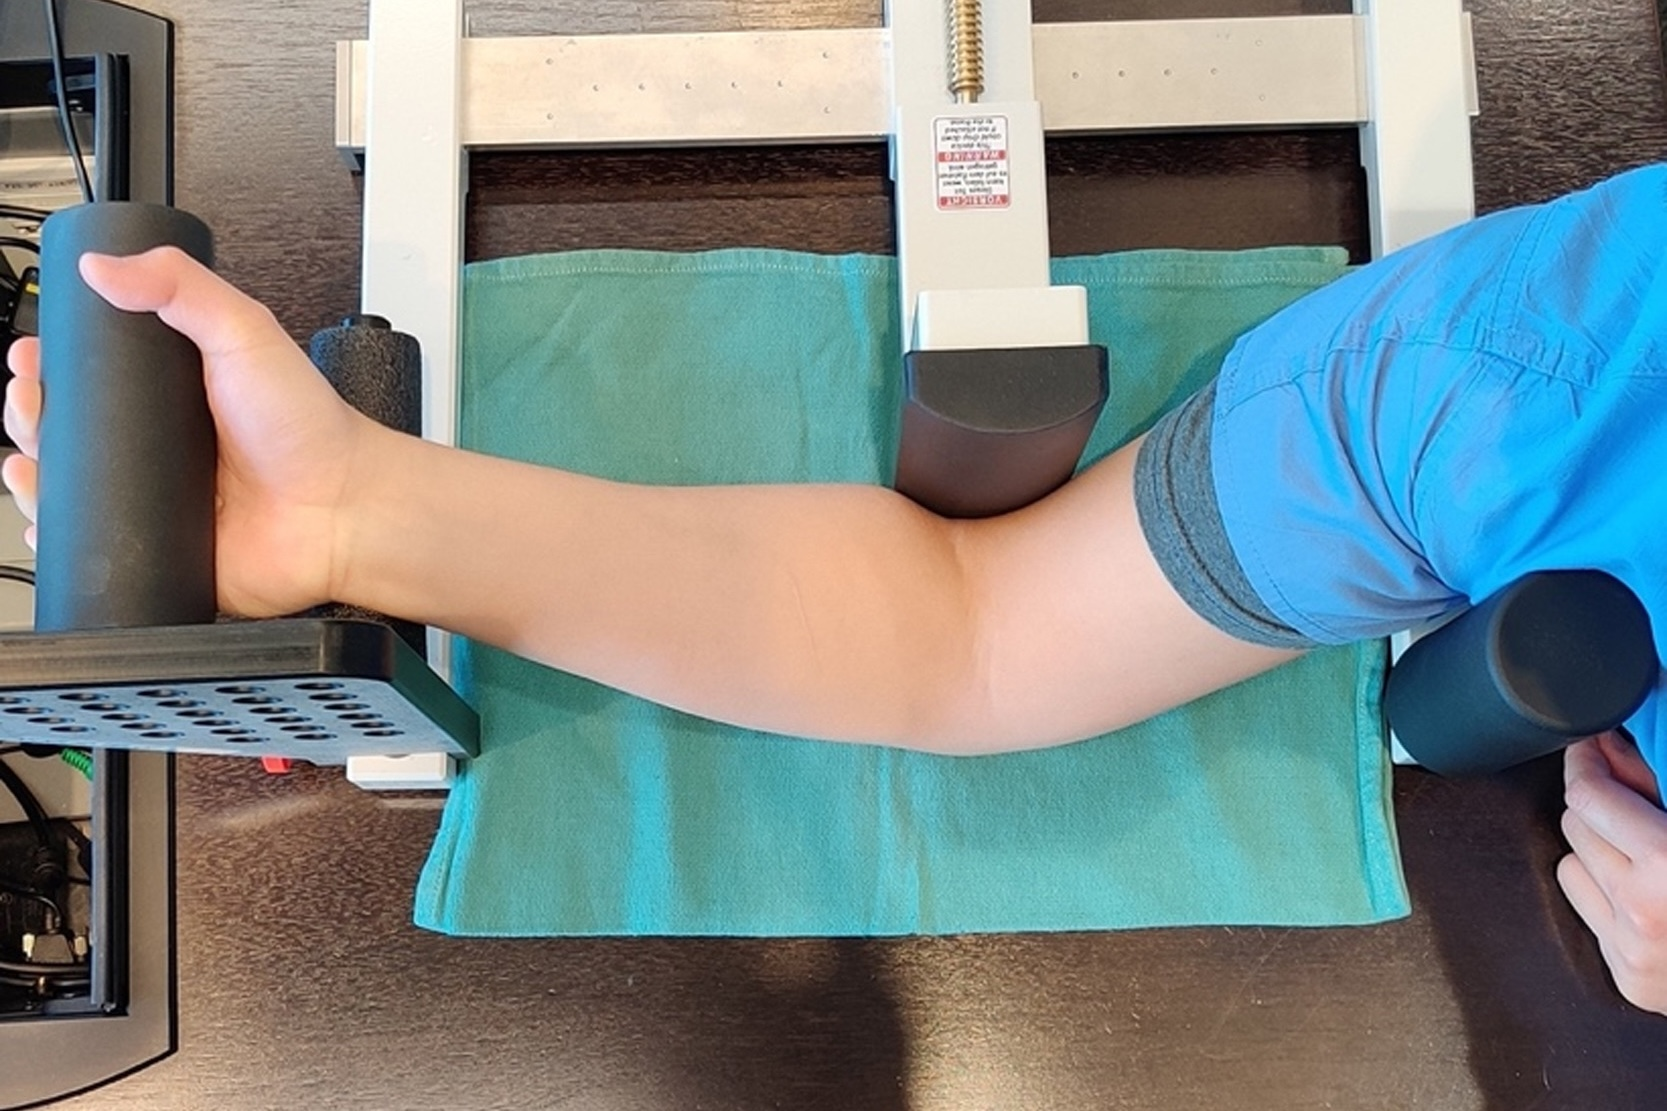
\includegraphics[width = 0.5\linewidth]{elbow_ultrasound.jpg}\\
    {\scriptsize from Gupta et al. (2023)}
  \end{frame}

  \begin{frame}{\bf Thank You!}
    \begin{center}
      \href{https://saberpowers.com/research}{saberpowers.com/\alert{\bf research}}
    \end{center}
  \end{frame}

\end{document}
